%システムモデルと処理の手順の解説

%1st paragraph
%1システム図にある、大きなモジュールの紹介
Fig.~\ref{system} shows the system model of the proposed system, which comprises sensor devices, an edge computer, and a GPU server. 
    \deleted{%1-1Sensor device
    The sensor device includes a LiDAR unit and an edge device.}
    \deleted{%1-2Edge computer
    The edge computer consists of a receiver and a merger.}
    \deleted{%1-3GPU server
    The GPU server comprises a trimmer, a feature estimator, and processors for classification.}
    \deleted{        %1-3-1The processor for classification
        The processors for classification consist of a clustering part, downsampling part, normalizing part, and classifying part.}
    \revised{Each sensor device has a LiDAR unit and an edge device; the edge computer has a receiver and a merger; the GPU server has a trimmer, a feature estimator, and classification processors with clustering, downsampling, normalizing, and classifying parts.}

\begin{deletedblock}
%2nd paragraph
%1LiDARによるデータ取得
In the sensor device, the LiDAR unit acquires a stream of 3D data. 
%2Edge deviceのデータ格納
The edge device stores the stream of 3D data from the LiDAR unit. 
%3Edge computerのデータ受け取り
In the edge computer, the receiver performs reception of the 3D data from the multiple sensor devices. 
%4Edge computerのデータのマージ
The merger aggregates the received 3D data into an aggregated 3D data. 
%5GPUサーバーによるデータ処理
The GPU server processes the aggregated 3D data. 
%6点群のトリミング
The trimmer performs trimming for a region where a person exists from the point cloud of each frame of the aggregated 3D data. 
%7点特徴の抽出
The feature estimator extracts point features from the trimmed point clouds. 
%8クラスタリング
In the GPU server, the clustering part removes the extra points in the calibrated point clouds. 
%9ダウンサンプリング
The downsampling part reduces the number of points in the clustered point clouds. 
%10正規化
The normalizing part performs normalization for the coordinates of the downsampled point clouds. 
%11ディープラーニングによる分類
The classifying part performs the classification for the normalized point clouds using the extracted point features. 
\end{deletedblock}
%2
\revised{3D data are acquired by each LiDAR unit, stored on the edge device, received and merged by the edge computer, and processed on the GPU server through trimming, feature extraction, clustering, downsampling, normalization, and classification.}

\begin{figure}[t]
  \centering
  {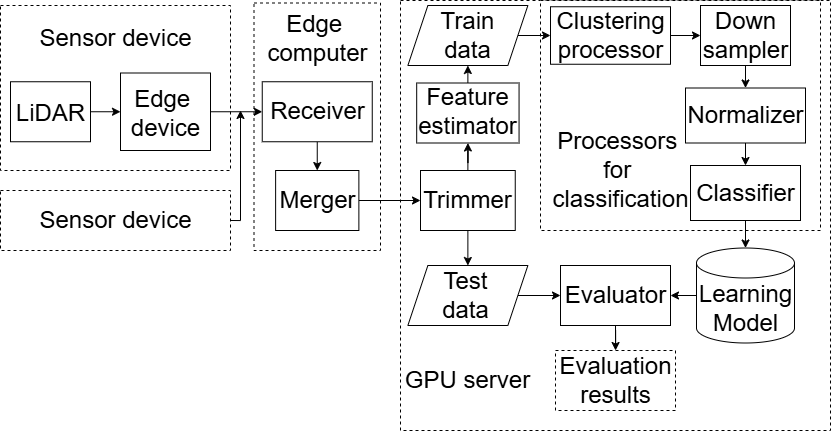
\includegraphics[width=\linewidth]{img/journal_system8.drawio.png}}
  \caption{System model.}
  \label{system}
\end{figure}
